\chapter{Resultados con el modelo de Drude-Sommerfeld}

%
%\section{Resultados con el modelos de Drude-Sommerfeld}
%	\subsection{Variación de parámetros}
%	\subsection{Conservación de la energía en el sistema}
%\section{Simulaciones con materiales reales}
%	\subsection{Variacionde parámetros}
%	


Para estudiar la respuesta electromagnética (EM) de una monocapa de nanopartículas (NPs) inmersa en un medio dieléctrico, denominado matriz, y soportada sobre un sustrato dieléctrico, se emplea el formalismo del modelo de esparcimiento coherente (Coherent Scattering Model, CSM) para calcular la reflectanci $R$ y transmistancia $T$ del sistema. El CSM que proporciona expresiones analíticas de los coeficientes de amplitud de reflexión $r$ y transmisión $t$ de la monocapa cuando está suspendida en el espacio libre (Free Stanting Monolayer, FSM) [Ecs. \eqref{eqs:rtcoh}], y para el sistema matriz-monocapa-sustrato tanto en incidencia externa [Ecs. \eqref{eqs:rtCSMext}] como en una configuración de reflexión total atenuada \index{Reflexión total!atenuada} (Attenuated Total Reflection, ATR) [Ecs. \eqref{eqs:rtCSMATR}]. La función dieléctrica $\varepsilon(\omega)$, en este capítulo, de las NPs que conforman a la monocapa se describe mediante el modelo de Drude-Sommerfeld [Ec. \eqref{eq:Drude}], dado que depende sólo de dos parámetros: la frecuencia de plasma $\omega_p$ y la constante fenomenológica de amortiguamiento $\gamma$. Mediante la elección de los parámetros $\omega_p$ y $\gamma$ es posible sintonizar las resonancias plasmónicas de superficie (Surface Plasmon Resonances, SPRs) así como ajustar el ancho de cada una de ellas, evitando así el traslape y facilitando la identificación de cada modo de manera individual. De esta forma, es posible identificar la presencia de algún otro modo como el reportado en \cite{kabashin2009plasmonic} y \cite{danilov2018ultra}, que es distinto a las SPRs de partículas individuales (Single Particles SPR, SP-SPRs) .	En la primera sección se analiza la reflectancia de una FSM esto es, empleando el modelo de Drude-Sommerfled en un primer caso con parámetros $\omega_p = 4.3$ eV y  $\gamma = 0.15$ eV [ver Fig. \ref{sfig:Drude4eV}], y en un segundo caso con $\omega_p = 10$ eV y $\gamma = 0.15$  [ver Fig. \ref{sfig:Drude10eV}]. Posteriormente, en la segunda sección, se estudia la reflectancia de una monocapa soportada en configuración de reflexión interna (Attenuated Total Reflection, ATR), ver Fig. \ref{fig:ATR1}, empleando el modelo de Drude-Sommerfeld y variando los parámetros de la monocapa: la fracción de cubierta $\Theta$ y radio de las NPs $a$.
	
	\section{Reflectancia de una monocapa suspendida en aire}
	
Para el cálculo de la reflectancia mediante el CSM de una FSM suspendida en aire ($n_m=1$), se empleó la Ec.  \eqref{eq:R} con el coeficiente de amplitud de reflexión coherente $r_{coh}$ [Ec.  \eqref{seq:rcoh}].  En la Fig.  \ref{fig:R-FSM} se muestran los resultados de la reflectancia $R$ como función del ángulo de incidencia $\theta_i$ y tanto de la longitud de onda $\lambda$ del haz incidente (escala inferior), así como de la energía del haz incidente en unidades de $\hbar\omega = h c /\lambda$ (escala superior).  La frecuencia de plasma empleada para la función dieléctrica tipo Drude fue $\omega_p = 4. 3$ eV y la constante fenomenológica de amortiguamiento $\gamma = 0. 15$ eV (que corresponden a $288. 5$ nm  y $8,270$ nm respectivamente). Se consideraron NPs de radio $a=30$ nm y fracciones de cubierta $\Theta$: $0. 05$, $0. 1$, $0. 2$, $0. 3$ y $0. 4$. En el renglón superior de la Fig. \ref{fig:R-FSM}, gráficas de $\mathbf{i)}$ a $\mathbf{v)}$, se muestra la reflectancia para polarización \emph{p}, mientras que en el renglón inferior se presentan las gráficas, de $\mathbf{vi)}$ a $\mathbf{x)}$, de la reflectancia para polarización \emph{s}. La línea punteada vertical verde  en $\lambda \approx 526$ nm corresponde a la SP-SPR de partícula individual dipolar ($\ell = 1$), mientras que la línea vertical rosa punteada en $\lambda \approx 462$ nm corresponde a la excitación del modo cuadrupolar ($\ell=2$).
					
	\begin{figure}[h!]\centering
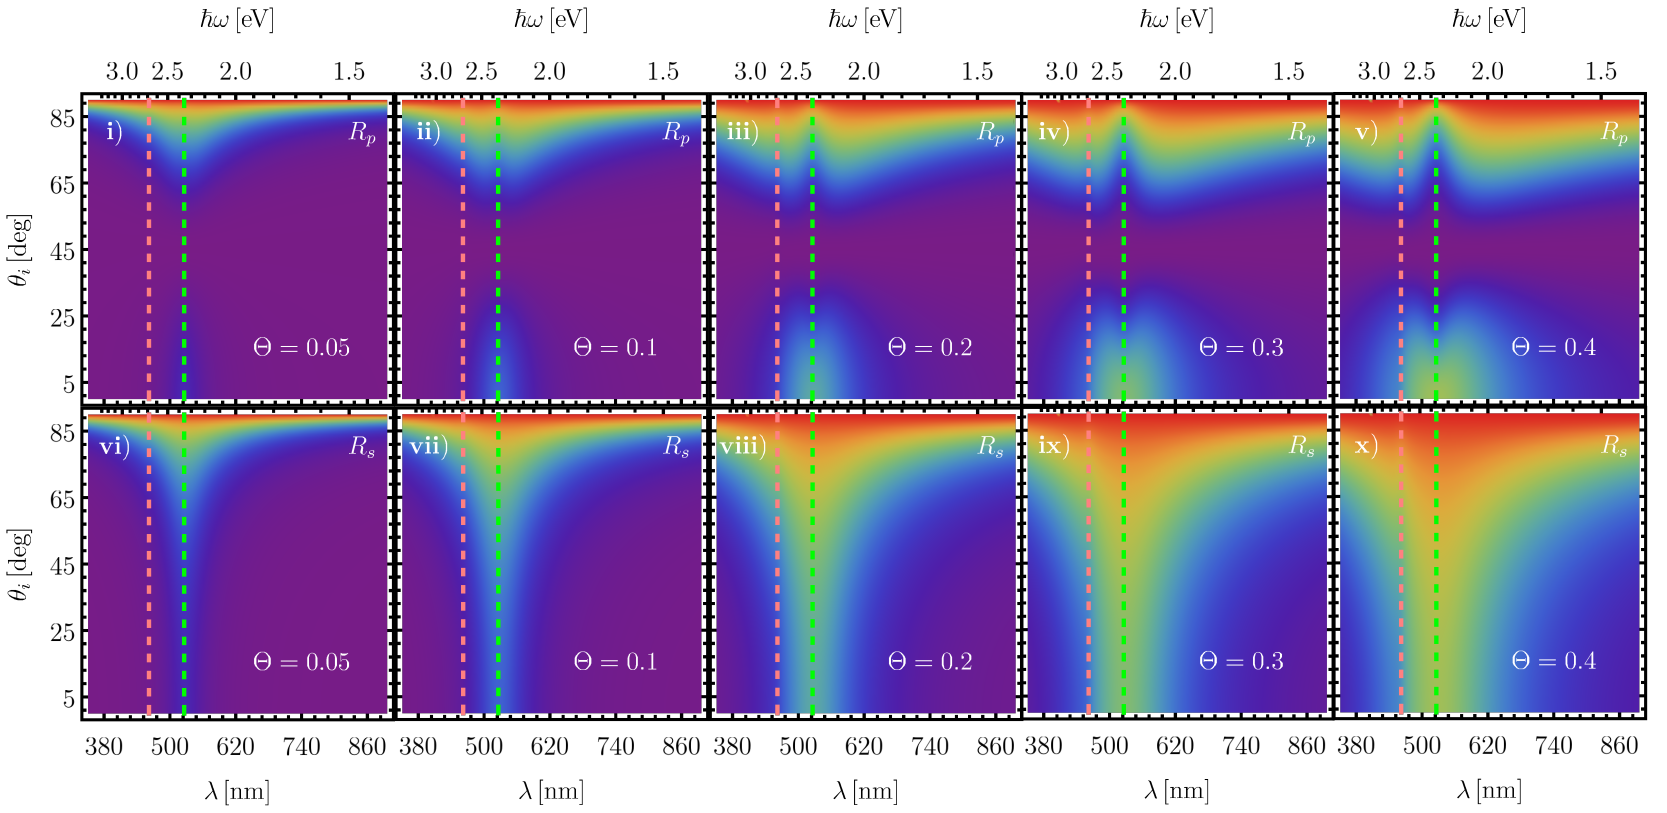
\includegraphics[width = .9\linewidth	]{2-Resultados/figs/4-Wp4FSMThetaVar/0-2D_Grid.png}%
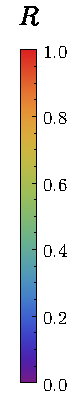
\includegraphics[scale=.85, trim={00 -5 00 00}, clip]{2-Resultados/figs/0-RBar_v}\vspace*{-1em}
	\caption{Gráficas de reflectancia para una FSM como función del ángulo de incidencia $\theta_i$ y tanto de la longitud de onda $\lambda$ (escala inferior), como de la energía del haz incidente en unidades de $\hbar\omega$ (escala superior), para una función dieléctrica tipo Drude con $\omega_p=4. 3$ eV  y  $\gamma=0. 15$ eV.  Las gráficas   en el renglón superior [$\mathbf{i)-v)}$]  muestran los resultados de reflectancia para  polarización \emph{p} y las del renglón inferior  [$\mathbf{i)-v)}$] para polarización  \emph{s}, donde se consideraron NPs de radio $a=30$ nm y distintas fracciones de cubierta $\Theta$: $0. 05$, $0. 1$, $0. 2$, $0. 3$ y $0. 4$. Las líneas verticales punteadas verdes y rosas corresponden a las SP-SPRs dipolar ($526$ nm) y cuadrupolar ($462$ nm), respectivamente.}	\label{fig:R-FSM}	
	\end{figure}						
					
La reflectancia para polarización \emph{p} [Fig. \ref{fig:R-FSM} $\mathbf{i)-v)}$] es cero para el ángulo de Brewster $\theta_B \approx 56^\circ$ y para regiones alejadas de las SP-SPRs (líneas punteadas verticales verde y rosa  localizadas en $526$ nm y $462$ nm, respectivamente). En la gráfica \textbf{v)}, $\Theta=0.4$,  se observa a $526$ nm (escala inferior) extinción de luz alrededor y, en la región al rededor de esta longitud de onda, la reflectancia comienza a aumentar. Conforme la fracción de cubierta disminuye, gráficas \textbf{iii)} y \textbf{iv)}, la extinción de luz es  menos evidente en $526$ nm y para las fracciones de cubierta $\Theta=0.05$ y $0.1$, gráficas \textbf{i)} y \textbf{ii)}, ya no es apreciable la extinción de luz a la frecuencia de la SP-SPR dipolar. En contraparte, para polarización \emph{s} [Fig. \ref{fig:R-FSM} $\mathbf{vi)-x)}$] la reflectancia es apreciable para todo ángulo de incidencia a las frecuencias de las SP-SPRs . Para ambas polarizaciones se observa que mientras la fracción de cubierta aumenta,  crece la región donde la reflectancia es apreciable, así como los valores calculados de $R$, evidenciando la presencia de las NPs en la monocapa.

En la Fig. \ref{fig:FSM-Cuts} se muestran cortes de la reflectancia graficada en la Fig. \ref{fig:R-FSM} para un ángulo de incidencia $\theta_i = 65^\circ$, tanto para un haz incidente con polarización \emph{p} [Fig. \ref{sfig:FSM-cutp}], como uno con polarización \emph{s} [Fig. \ref{sfig:FSM-cuts}]. Para la polarización \emph{p} se presenta un mínimo en la reflectancia alrededor de $526$ nm para fracciones de cubierta mayores a $\Theta = 0.05$. Los mínimos de $R_p$ a la frecuencia de la SP-SPR dipolar son más pronunciados conforme aumenta la fracción de cubierta. El cálculo  de $R_p$ para $\Theta=0.05$ se analiza en la gráfica interior de la Fig \ref{sfig:FSM-cutp}, en donde se observa un máximo en lugar de un mínimo en $R_p$. Para polarización \emph{s}, se presenta un máximo en la reflectancia a $526$ nm para todos los valores de $\Theta$. Para las fracciones de cubierta mayores, $\Theta = 0.3$ y $\Theta = 0.4$,  se observa un  mínimo en la reflectancia alrededor de $462$ nm para ambas polarizaciones, lo que corresponde a la SP-SPR cuadrupolar.

	\begin{figure}[h!]\centering
	\begin{subfigure}{.01\linewidth}\caption{}\label{sfig:FSM-cutp}\vspace{3.75cm}\end{subfigure}\hspace*{-.5em}
	\begin{subfigure}{.45\linewidth}\centering 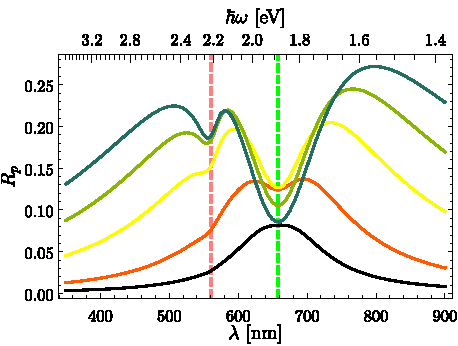
\includegraphics[scale=.75 ]{2-Resultados/figs/4-Wp4FSMThetaVar/cut_angle_65_p.pdf}\end{subfigure}
	\begin{subfigure}{.01\linewidth}\caption{}\label{sfig:FSM-cuts}\vspace{3.75cm}\end{subfigure}\hspace*{-.5em}
	\begin{subfigure}{.45\linewidth}\centering 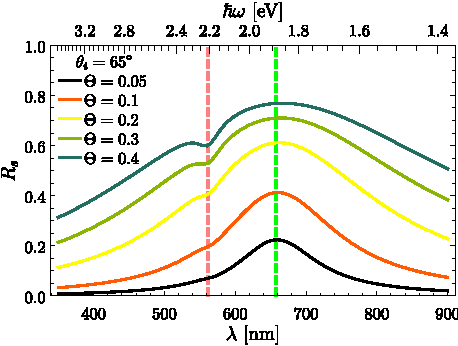
\includegraphics[scale=.75 ]{2-Resultados/figs/4-Wp4FSMThetaVar/cut_angle_65_s.pdf}\end{subfigure}\vspace*{-.5em}
	\caption{Cortes de la Fig. \ref{fig:R-FSM} a $\theta_i = 65^\circ$ de reflectancia de una FSM de NPs esféricas de radio $a=30$ nm en polarización \textbf{a)} \emph{p} y \textbf{b)} \emph{s} como función tanto de la longitud de onda $\lambda$ (escala inferior), como de la energía del haz incidente en unidades de $\hbar\omega$ (escala superior). Los parámetros de la función dieléctrica tipo Drude para las NPs son $\omega_p = 4.3$ eV y $\gamma = 0.15$ eV y las fracciones de cubierta consideradas fueron $\Theta$: $0. 05$, $0. 1$, $0. 2$, $0. 3$ y $0. 4$. Las líneas verticales punteadas verdes y rosas corresponden a las SP-SPRs dipolar ($526$ nm) y cuadrupolar ($462$ nm), respectivamente.}\label{fig:FSM-Cuts}
	\end{figure}	

En las Figs. \ref{fig:R-FSM} y \ref{fig:FSM-Cuts} se observa la respuesta EM de una monocapa de NPs suspendida en vacío al interactuar con una onda plana. Si se considera la presencia de un sustrato que soporte la monocapa, se puede estar en configuraci\'on de incidencia externa o interna seg\'un sea el medio de incidencia del haz de luz. Para incidencia externa, a todo ángulo de incidencia,  el haz que ilumina a las NPs es una onda plana, por lo que la posición de lo máximos y mínimos de la reflectancia no cambiarán y los valores de $R$ presentarán un decrecimiento respecto a los cálculos de la reflectancia para una FSM. Por otro lado, para el caso de incidencia interna y ángulos mayores al ángulo crítico $\theta_c = \arcsin(n_m/n_s)$, las NPs en la monocapa son iluminadas por ondas evanescentes, y es posible excitar los plasmones de superficie en las NPs a frecuencias específica, a las cuales, el valor de la reflectancia es menor que la unidad, es decir, se estaría en una configuración de reflexión total atenuada (Attenuated Total Reflection, ATR).

	\subsection{Reflectancia de una monocapa en configuración ATR}

La respuesta EM de una monocapa de NPs suspendida en una matriz con índice de refracción $n_m$ y soportada por un sustrato con índice de refracción $n_s$, se calcula al emplear la Ec.  \eqref{eq:R} con el coeficiente de amplitud de reflexión $r$ de la Ec.  \eqref{eq:r3CSM}. Para comparar los resultados de la reflectancia $R$ para una FSM y una monocapa en configuración ATR, se emplean los parámetros utilizado en los cálculos de las Figs. \ref{fig:R-FSM} y \ref{fig:FSM-Cuts} ($n_m=1$ , $a=30$ nm, $\omega_p=4.3$ eV y  $\gamma = 0.15$ eV) considerando un sustrato con índice de refracción $n_s=1.5$. En la Fig.  \ref{fig:R-ATR4} se presentan los resultados de la reflectancia $R$ como función del ángulo de incidencia $\theta_i$ y tanto de la longitud de onda $\lambda$ del haz incidente (escala inferior), así como de la energía del haz $\hbar\omega$ (escala superior). Los resultados para polarización \emph{p} se muestran en las gráficas $\mathbf{i)-v)}$ en la Fig.  \ref{fig:R-ATR4} y para polarización \emph{s} en las gráficas $\mathbf{vi)-x)}$. Al igual que para la FSM, se consideraron los casos para la fracción de cubierta $\Theta = 0.05,\,0.1,\,0.2,\,0.3$ y $0.4$. Las SP-SPRs corresponden a la línea vertical verde punteada en $\lambda \approx 526$ nm para el modo dipolar y la línea vertical rosa punteada en  $\lambda \approx 462$ nm para el modo cuadrupolar. Adicionalmente, los puntos amarillos en la Fig. \ref{fig:R-ATR4} corresponden a los mínimos en $R$ para ángulos mayores a $\theta_c\approx 41^\circ$ y longitudes de onda mayores a la SP-SPRs dipolar.

	\begin{figure}[h!]\centering
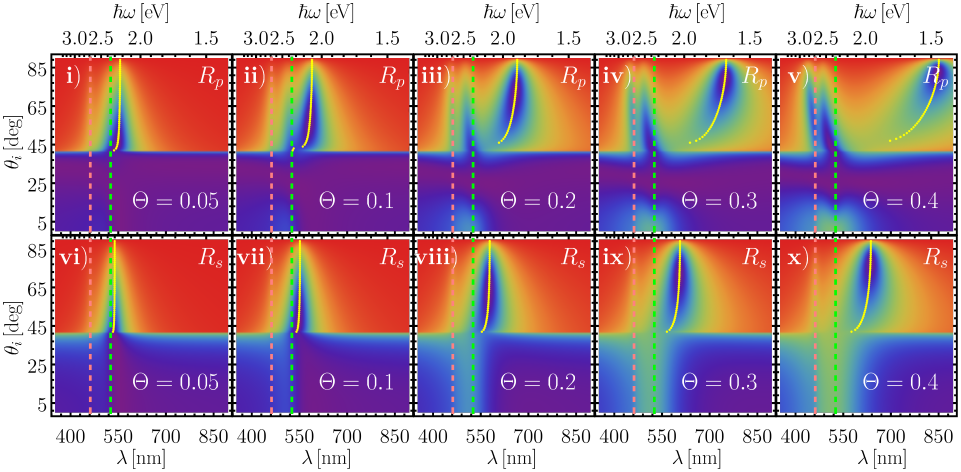
\includegraphics[width = .9\linewidth, trim={00 00 00 00}, clip	]{2-Resultados/figs/1-Wp4ThetaVar/0-2D_Grid}%
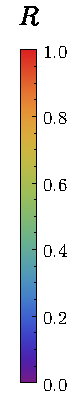
\includegraphics[scale=.85, trim={00 -5 00 00}, clip]{2-Resultados/figs/0-RBar_v}
	\caption{Gráficas de reflectancia de una monocapa en configuración ATR como función del ángulo de incidencia $\theta_i$ y de la longitud de onda $\lambda$ (escala inferior), así como de la energía del haz incidente en unidades de $\hbar\omega$ (escala superior), para una función dieléctrica tipo Drude con $\omega_p=4. 3$ eV  y  $\gamma=0. 15$ eV.  Las gráficas   en el renglón superior [$\mathbf{i)-v)}$]  muestran los resultados de reflectancia para  polarización \emph{p} y las del renglón inferior  [$\mathbf{vi)-x)}$] para polarización  \emph{s}, donde se consideraron NPs de radio $a=30$ nm y distintas fracciones de cubierta $\Theta$: $0. 05$, $0. 1$, $0. 2$, $0. 3$ y $0. 4$. Las líneas verticales punteadas verdes y rosas corresponden a las SP-SPRs dipolar ($526$ nm) y cuadrupolar ($462$ nm), respectivamente.	os puntos amarillos corresponden a los mínimos en $R$ para ángulos mayores a $\theta_c\approx 41^\circ$ y longitudes de onda mayores a la SP-SPRs dipolar.}	\label{fig:R-ATR4}	
	\end{figure}	


En la Fig.  \ref{fig:R-ATR4} la reflectancia para ángulos mayores al ángulo crítico, $\theta_c \approx 41^\circ $ para una interfaz vidrio-aire, es igual a la unidad excepto en dos regiones: alrededor de las longitudes de onda correspondientes a las SP-SPRs (líneas punteadas verticales) y en una región a longitudes de onda mayores a la SP-SPR dipolar (puntos amarillos). La disminución en la reflectancia después del ángulo crítico alrededor de las SP-SPRs es resultado de la extinción debido a las NPs y, al considerar la interacción entre ellas, así como con el sustrato, puede presentarse un corrimiento al rojo, o al azul, de la SPR que, además, depende del ángulo de incidencia del haz, como se observa en las gráficas \textbf{iii)--v)}. La extinción a las longitudes de onda cercanas a las SP-SPRs es más evidente para las fracciones de cubierta más grandes consideradas, por ejemplo, en el panel superior de la Fig. \ref{fig:R-ATR4}, la reflectancia $R_p$ toma valores más cercanos al cero en la gráfica $\mathbf{v)}$, $\Theta = 0.4$,  en comparación a la gráfica $\mathbf{i)}$, $\Theta = 0.05$. A pesar de que este comportamiento es análogo para la polarización \emph{s}, panel inferior de la  Fig. \ref{fig:R-ATR4}, los valores de $R_s$ a las frecuencias de las SP-SPRs son mayores que los de $R_p$, como se observa al comparar las gráficas de los cálculos con $\Theta=0.3$ \textbf{iv)}, $R_p$, y \textbf{ix)}, $R_s$.


Adicional a la región cercana a las SP-SPRs, se observa una región en donde la luz es reflejada con una intensidad, relativa a la intensidad del haz incidente, menor a la unidad, que corresponde a los puntos amarillos en los mínimos de la reflectancia para ángulos de incidencia mayores al ángulo crítico y para longitudes de onda mayores a la SP-SPR dipolar. La separación entre las SP-SPRs y los mínimos a longitudes de ondas mayores (puntos amarillos) aumenta conforme lo hace la fracción de cubierta $\Theta$; este comportamiento es más evidente en polarización \emph{p} que en \emph{s} [ver \textbf{v)} y \textbf{x)} en la Fig.  \ref{fig:R-ATR4}].  Dado que los puntos amarillos corresponden a una excitación que ocurre energías  menores en comparación a las de partículas individuales, se especula que la excitación se debe a una respuesta colectiva como la PSLR reportada en \cite{danilov2018ultra}.
  
  En la Fig. \ref{fig:R-ATR4-Cuts} se presentan cortes para $\theta_i = 65^\circ$ de la reflectacia graficada en la Fig. \ref{fig:R-ATR4} para todas las fracciones de cubierta consideradas; las líneas punteadas verticales corresponden a las longitudes de onda de las SP-SPRs (verde para la excitación dipolar y rosa para la cuadrupolar). En polarización \emph{p}, Fig. \ref{sfig:R-ATR4-cutp}, la excitación de la monocapa para $\Theta=0.05$ alrededor de $\lambda \approx 462$ nm coincide con la SP-SPR cuadrupolar y conforme la fracción de cubierta aumenta, la excitación de la monocapa presenta un corrimiento al azul. En polarización \emph{s}, Fig. \ref{sfig:R-ATR4-cuts},  la SP-SPR cuadrupolar se observa en la respuesta de la monocapa para todas las fracciones de cubierta. La reflectancia, para ambas polarizaciones, en la longitud de onda de la SP-SPR cuadrupolar disminuye conforme la fracción de cubierta crece, por lo que se relaciona con la cantidad de NPs presentes en la monocapa.
  
\begin{figure}[h!]\centering
	\begin{subfigure}{.01\linewidth}\caption{}\label{sfig:R-ATR4-cutp}\vspace{3.75cm}\end{subfigure}\hspace*{-.5em}
	\begin{subfigure}{.45\linewidth}\centering 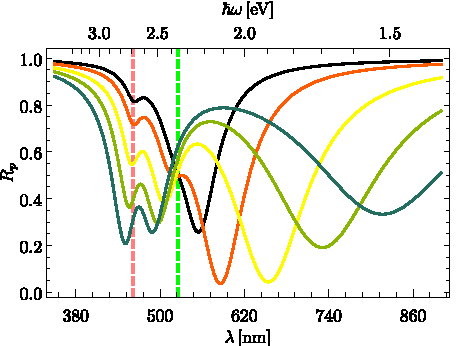
\includegraphics[scale=.75 ]{2-Resultados/figs/1-Wp4ThetaVar/cut_angle_65_p.pdf}\end{subfigure}
	\begin{subfigure}{.01\linewidth}\caption{}\label{sfig:R-ATR4-cuts}\vspace{3.75cm}\end{subfigure}\hspace*{-.5em}
	\begin{subfigure}{.45\linewidth}\centering 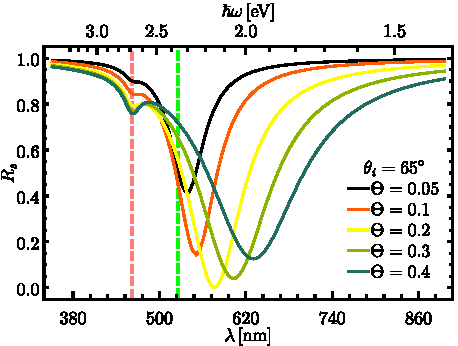
\includegraphics[scale=.75 ]{2-Resultados/figs/1-Wp4ThetaVar/cut_angle_65_s.pdf}\end{subfigure}\vspace*{-.5em}
	\caption{Cortes de la Fig. \ref{fig:R-ATR4} a $\theta_i = 65^\circ$ de reflectancia de una monocapa en configuración ATR de NPs esféricas de radio $a=30$ nm en polarización \textbf{a)} \emph{p} y \textbf{b)} \emph{s} como función de la longitud de onda $\lambda$ (escala inferior) y de la energía $\hbar \omega$ (escala superior). Los parámetros de la función dieléctrica tipo Drude para las NPs son $\omega_p = 4.3$ eV y $\gamma = 0.15$ eV y las fracciones de cubierta consideradas fueron $\Theta$: $0. 05$, $0. 1$, $0. 2$, $0. 3$ y $0. 4$. Las líneas verticales punteadas verdes y rosas corresponden a las SP-SPRs dipolar ($526$ nm) y cuadrupolar ($462$ nm), respectivamente.  }\label{fig:R-ATR4-Cuts}
	\end{figure}	  
    
A diferencia de la SP-SPR cuadrupolar, la excitación dipolar de partícula individual ($526$ nm) no es observable para todos los casos presentados en la Fig. \ref{fig:R-ATR4-Cuts}. En la respuesta óptica de la monocapa sólo se presenta una excitación cercana a la SP-SPR dipolar para los resultados de $R_p$ y para las fracciones de cubierta $\Theta = 0.1,\,0.2,\,0.3$ y $0.4$. Esta excitación se corre al azul conforme $\Theta$ aumenta, al igual que la SP-SPRs cadrupolar. Sin emabargo, se observa una excitación a longitudes de onda mayores a la SP-SPR dipolar para ambas polarizaciones.
 
Los mínimos a longitudes de onda mayores a $530$ nm, para ambas polarizaciones, presentan un corrimiento al rojo conforme la fracción de cubierta de la monocapa aumenta, contrario al comportamiento observado en las excitaciones de la monocapa cercanas a las SP-SPRs. Otra diferencia entre las excitaciones en $\lambda$ mayores a las SP-SPRs y los corrimientos al azul de éstas es que la disminución en el valor de $R$ no es monotona, sino que el decrecimiento en $R$ es máximo a fracciones de cubierta media, como $\Theta=0.2$, que es el valor donde la reflectancia es menor. Por lo anterior, los mínimos en $R_p$ y $R_s$ localizados a longitudes de onda mayores a la de los modos plasmónicos de partícula individual no son corrimientos de las excitaciones multipolares de una partícula, sino que se asocian a una respuesta colectiva de las NPs en la monocapa, más apreciable para la polarización \emph{p} que para \emph{s}.

Es posible separar las resonancias del presunto modo colectivo de las SP-SPRs al incrementar la frecuencia de plasma en el modelo de Drude, que caracteriza la respuesta EM de las NPs. Al considerar $\omega_p = 10$ eV las SP-SPRs se corren al azul, por lo que pueden distinguirse del presunto modo colectivo. Los resultados de la reflectancia de un sistema monocapa con los parámetros empleados en la Fig. \ref{fig:R-ATR4}, pero con $\omega_p = 10$ eV, se muestran en la Fig. \ref{fig:R-ATR10}. Adicional a la SP-SPR dipolar y cuadrupolar (líneas verticales punteadas verde y rosa en $265$ nm y $211$ nm, respectivamente), la SP-SPR octopolar ($\ell = 3$) se muestra en las gráficas mediante la línea vertical punteada azul en $195$ nm, al igual que el presunto modo colectivo que corresponde a los puntos amarillos.
	
  	\begin{figure}[h!]\centering
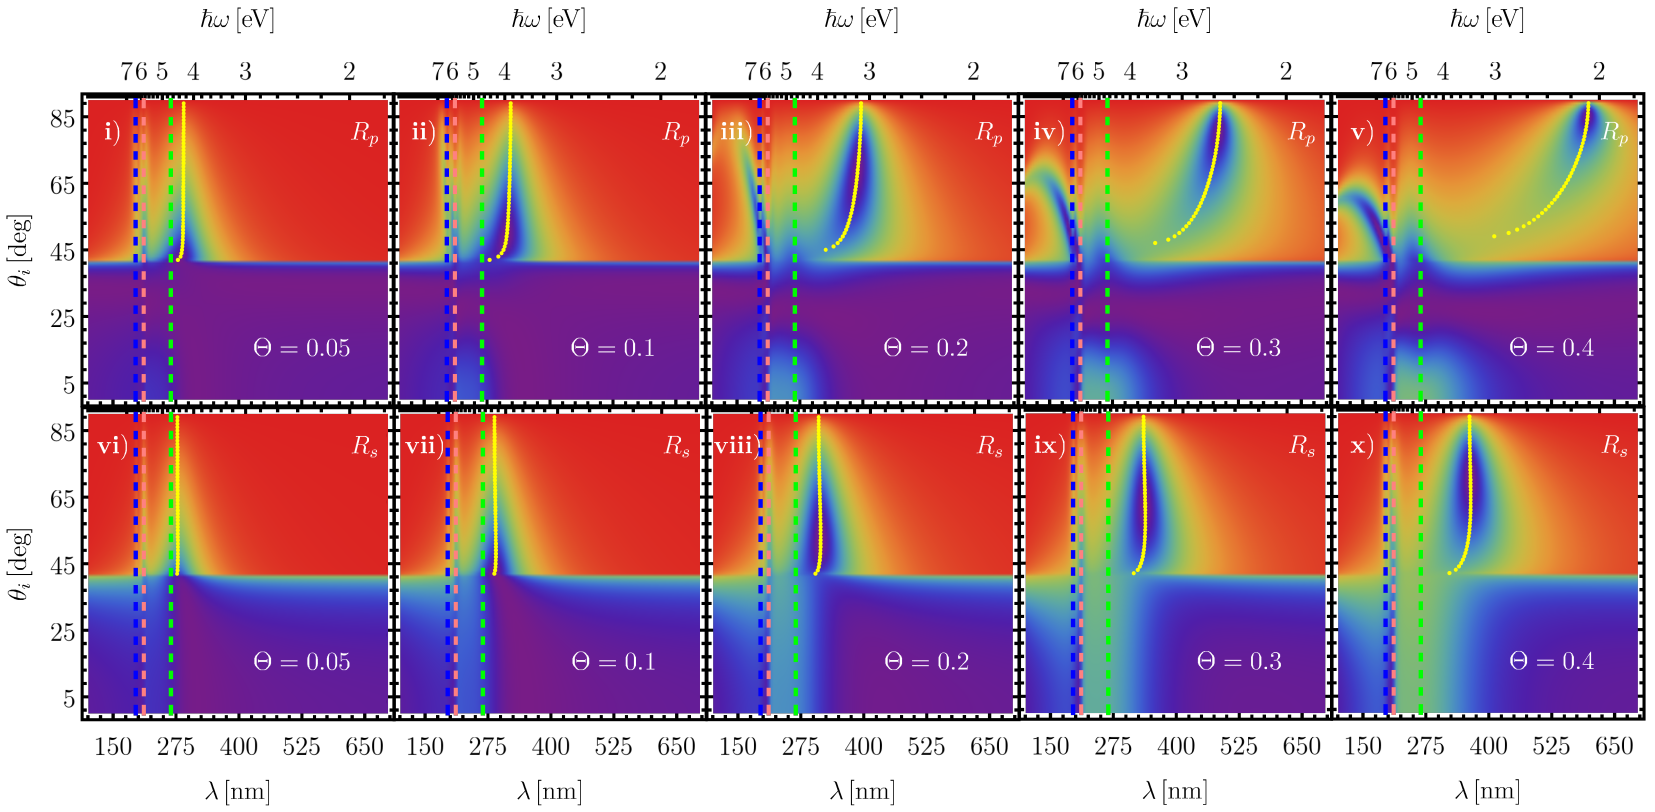
\includegraphics[width = .9\linewidth]{2-Resultados/figs/2-Wp10ThetaVar/0-2D_Grid.png}%
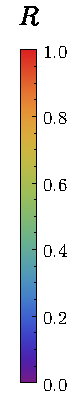
\includegraphics[scale=.85, trim={00 -5 00 00}, clip]{2-Resultados/figs/0-RBar_v}
	\caption{Gráficas de reflectancia de una monocapa en configuración ATR como función del ángulo de incidencia $\theta_i$ y de la longitud de onda $\lambda$ (escala inferior), así como de la energía del haz incidente en unidades de $\hbar\omega$ (escala superior), para una función dieléctrica tipo Drude con $\omega_p=10$ eV  y  $\gamma=0. 15$ eV.  Las gráficas   en el renglón superior [$\mathbf{i)-v)}$] muestran los resultados  para  polarización \emph{p} y las del renglón inferior  [$\mathbf{vi)-x)}$] para polarización  \emph{s}, donde se consideraron NPs de radio $a=30$ nm y distintas fracciones de cubierta $\Theta$: $0. 05$, $0. 1$, $0. 2$, $0. 3$ y $0. 4$. Las líneas verticales punteadas verdes, rosas y azules corresponden a las SP-SPRs dipolar ($265$ nm), cuadrupolar ($211$ nm) y octopolar ($195$ nm), respectivamente.  Los puntos amarillos corresponden a los mínimos en $R$ para ángulos mayores a $\theta_c\approx 41^\circ$ y longitudes de onda mayores a la SP-SPRs dipolar. }	\label{fig:R-ATR10}	
	\end{figure}		
	
	
En las gráficas mostradas en la Fig. \ref{fig:R-ATR10} son apreciables dos regiones de valores mínimos para $R$, también observadas en el caso de NPs con una función dieléctrica con el parámetro $\omega_p=4.3$ eV: valores de $\lambda$ cercanos a las SP-SPRs (líneas verticales punteadas) y la excitación a energías menores (puntos amarillos). Sin embargo, para los casos de polarización \emph{p} y $\Theta = 0.2,\,0.3$ y $0.4$, gráficas \textbf{iii)} a \textbf{v)}, se observa una tercera región con mínimos locales en la reflectancia, localizada en valores de $\lambda$ menores a la SP-SPR cuadrupolar y a distintos ángulos de incidencia, la cual adopta la forma de una ramificación que se corre al azul conforme el ángulo de incidencia aumenta. Para polarización \emph{s}, se observa una franja entre las SP-SPRs cuadrupolar y octopolar en donde $R$ toma valores menores que en las longitudes de onda de la excitación de partícula individual. Para todos los casos defracción de cubierta y polarización, la separación  entre el presunto modo colectivo (puntos amarillos) y las longitudes de onda correspondientes a las SP-SPRs aumenta conforma lo hace la fracción de cubierta, comportamiento observado para $\omega_p = 4.3$ eV, en la Fig.  \ref{fig:R-ATR4}.  Asimismo, esta separación es mayor para la polarización \emph{p} que para la polarización \emph{s}, por lo que el comportamiento es análogo al observado en la Fig. \ref{fig:R-ATR4}. Adicionalmente, al haber cambiado la frecuencia de plasma se logró aumentar la distancia entre las SP-SPRs y el presunto modo colectivos (ver. \ref{fig:R-ATR4} y \ref{fig:R-ATR10}) , es decir, este modo es sintonizable.

En la Fig. \ref{fig:R-ATR10-Cuts} se muestra la reflectancia para la polarización \emph{p}, Fig. \ref{sfig:R-ATR10-cutp}, y polarización \emph{s}, Fig. \ref{sfig:R-ATR10-cuts}, como función de la longitud de onda, para el ángulo $\theta_i = 65^\circ$ para una monocapa de NPs y fracciones de cubierta consideradas en la Fig. \ref{fig:R-ATR10}; las líneas punteadas verde, rosa y azul corresponden a las SP-SPRs dipolar, cuadrupolar y octopolar respectivamente. Para ambas polarizaciones y para todas las fracciones de cubierta, se presenta una excitación a la longitud de onda correspondiente a la SP-SPR octopolar, al igual que un corrimiento al azul de la SP-SPR cuadrupolar. Adicional a estas excitaciones, en polarización \emph{p} se observa una excitación que se localiza en la longitud de onda de la SP-SPR cuadrupolar para $\Theta=0.05$ y se corre al azul conforme aumenta la fracción de cubierta, hasta localizarse en $\lambda= 135$ nm para $\Theta=0.4$. Esta excitación corresponde a la ramificación también presente en las gráficas \textbf{iii)} a \textbf{v)} de la Fig. \ref{fig:R-ATR10}. En polarización \emph{s} para $\Theta\geq 0.2$ se observa una segunda excitación cercana a la SP-SPR cuadrupolar, la cual corresponde a la franja observada en las gráficas \textbf{ix)} y \textbf{x)} de la Fig. \ref{fig:R-ATR10} entre las SP-SPR cuadrupolar y octopolar (líneas verticales punteadas rosa y azul), y que se corre al azul conforme aumenta la fracción de cubierta.

	\begin{figure}[h!]\centering
	\begin{subfigure}{.01\linewidth}\caption{}\label{sfig:R-ATR10-cutp}\vspace{3.75cm}\end{subfigure}\hspace*{-.5em}
	\begin{subfigure}{.45\linewidth}\centering 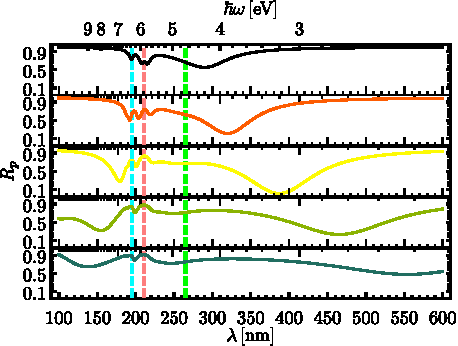
\includegraphics[scale=.75 ]{2-Resultados/figs/2-Wp10ThetaVar/cut_angle_65_p_Stack.pdf}\end{subfigure}
	\begin{subfigure}{.01\linewidth}\caption{}\label{sfig:R-ATR10-cuts}\vspace{3.75cm}\end{subfigure}\hspace*{-.5em}
	\begin{subfigure}{.45\linewidth}\centering 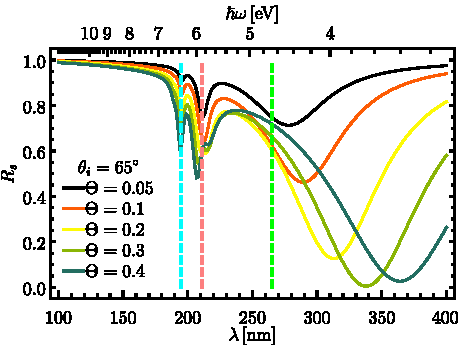
\includegraphics[scale=.75 ]{2-Resultados/figs/2-Wp10ThetaVar/cut_angle_65_s.pdf}\end{subfigure}\vspace*{-.5em}
	\caption{Cortes de la Fig. \ref{fig:R-ATR10} a $\theta_i = 65^\circ$ de reflectancia de una monocapa en configuración ATR de NPs esféricas de radio $a$ en polarización \textbf{a)} \emph{p} y \textbf{b)} \emph{s} como función de la longitud de onda $\lambda$ (escala inferior) y de la energía en unidades de $\hbar \omega$ (escala superior). Los parámetros de la función dieléctrica tipo Drude para las NPs son $\omega_p = 10$ eV y $\gamma = 0.15$ eV y las fracciones de cubierta consideradas fueron $\Theta$: $0. 05$, $0. 1$, $0. 2$, $0. 3$ y $0. 4$. Las líneas verticales punteadas verdes, rosas y azules corresponden a las SP-SPRs dipolar ($265$ nm), cuadrupolar ($211$ nm) y octopolar ($195$ nm), respectivamente.  }\label{fig:R-ATR10-Cuts}
	\end{figure}	

La resonancia dipolar de una partícula individual no se alcanza a distinguir en la Fig. \ref{fig:R-ATR10-Cuts} para ninguna polarización, en cambio, se presentan los mínimos atribuidos a una respuesta colectiva. Estas excitaciones se comportan de manera análoga al caso de $\omega_p = 4.3$ eV: se corren al rojo conforme aumenta la fracción de cubierta y su presencia es más evidente para fracciones de cubierta media, siendo  $\Theta=0.2$ para polarización \emph{p} y $\Theta=0.3$ para polarización \emph{s} cuando la reflectancia en la excitación del modo colectivo alcanza el valor mínimo de reflectancia. En la Fig. \ref{sfig:R-ATR10-cutp} y \ref{sfig:R-ATR10-cuts}  se observada qua excitación que se corre al azul a longitudes de onda menores a la SP-SPR octopolar es más evidente para $\Theta=0.2$, una fracción de cubierta media.

En las gráficas de la Fig. \ref{fig:R-ATR10-Cuts} no se distinguen las excitaciones correspondientes a la SP-SPR dipolar en la respuesta EM de la monocapa a pesar de que se aumentó el parámetro $\omega_p$ de $4.3$ eV a $10$ eV, sin embargo, la supuesta respuesta colectiva es apreciable para todas las fracciones de cubierta analizadas, por lo que se especula que el modo colectivo a caracterizar (puntos amarillos) se traslapa con la SP-SPR  dipolar. Adicionalmente, la distnacia entre el valor de la SP-SPR dipolar y la del presunto modo colectivo aumentó al cambiar $\omega_p$, por lo que éste puede ser sintonizado. Ya que se observó una segunda respuesta que no corresponde a las SP-SPRs, sino que sigue las tendencias del presunto modo colectivo, se especula que es un complemento  de ellas, dado que las  PSLRs reportadas en \cite{danilov2018ultra} son, para un sistema determinado, dos excitaciones que se corren al rojo y al azul. Es decir, que tanto el modo que se corre al azul a partir de la SP-SPR dipolar, como el presunto modo colectivo (puntos amarilos en la Fig. \ref{fig:R-ATR10}) se pueden relacionar con las PSLRs.  

 Ya que el presunto modo colectivo sufre un corrimiento al rojo al aumentar la fracción de cubierta, se analizó si el comportamiento es semejante a cambios en el radio $a$ de las NPs.  Este análisis se llevó a cabo dado que tanto el radio $a$ como la fracción de cubierta $\Theta$ modifican el volumen neto de material plasmónico, es decir, hay en la monocapa una mayor cantidad de electrones libres, corroborando que los mínimos en $R$  a energías menores que la de la SP-SPR dipolar, se deben a un efecto colectivo de las NPs, al igual que las PSLRs. Se consideró, al igual que en los casos pasados (ver. Figs. \ref{fig:R-ATR4} y  \ref{fig:R-ATR10}) que la matriz donde están suspendidas las NPs de radio $a$ es aire ($n_m = 1$), y el sustrato tiene un índice de refracción $n_m= 1.5$. La función dieléctrica de las NPs en la monocapa (con $\Theta=0.3$) está dada por una función tipo Drude [Ec. \eqref{eq:Drude}] con los parámetros $\omega_p =4.3$ eV y $\gamma=0.15$ eV. Los resultados de la reflectancia se muestran en la Fig.  \ref{fig:R-RVar}, como función del ángulo de incidencia, tanto de la longitud de onda $\lambda$ (escala inferior) como de la  energía $\hbar\omega$ (escala superior) del haz incidente. Se consideraron los valores para el radio $a$ los siguientes: $3$ nm, $5$ nm, $10$ nm y $20$ nm,  en polarización \emph{p} [en la Fig.  \ref{fig:R-RVar}, $\mathbf{i)-iv)}$] y en polarización \emph{s} [en la Fig.  \ref{fig:R-RVar}, $\mathbf{v)-viii)}$].  Las SP-SPRs dipolar y cuadrupolar corresponden a las líneas punteadas verde y rosa, respectivamente. Para $a = 3$ nm y $5$ nm la excitación dipolar se localiza en $\lambda\approx 500$ nm, para el radio  $a = 10$ nm en $\lambda\approx 503$ nm y $a=20$ nm en $\lambda\approx 512$ nm, mientras que la SP-SPR cuadrupolar se localiza en $456$ nm para $a\leq 10$ nm y para el caso  $a=20$ nm, $462$ nm.

	\begin{figure}[h!]\centering
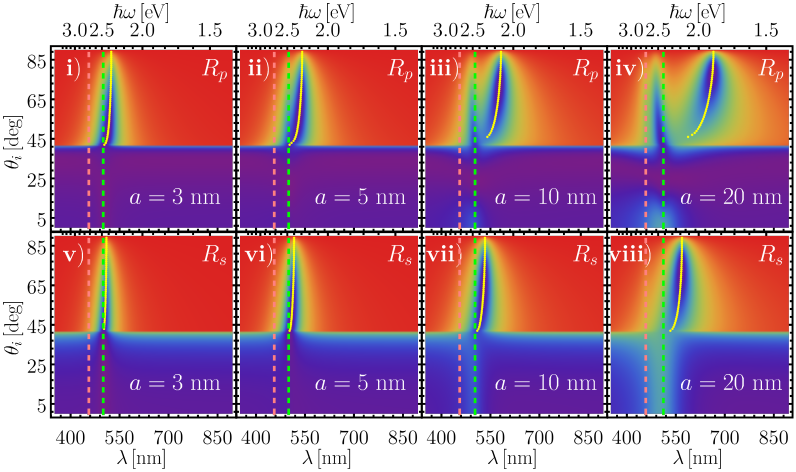
\includegraphics[width = .9\linewidth]{2-Resultados/figs/3-Wp4rVar/0-2D_Grid}%
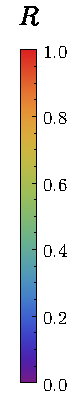
\includegraphics[scale=1, trim={00 -15 00 00}, clip]{2-Resultados/figs/0-RBar_v}
	\caption{Gráficas de reflectancia de una monocapa en configuración ATR como función del ángulo de incidencia $\theta_i$ y de la longitud de onda $\lambda$ (escala inferior), así como de la energía del haz incidente en unidades de $\hbar\omega$ (escala superior), para una función dieléctrica tipo Drude con $\omega_p=4.3$ eV  y  $\gamma=0. 15$ eV.  Las gráficas   en el renglón superior [$\mathbf{i)-v)}$] muestran los resultados para  polarización \emph{p} y las del renglón inferior  [$\mathbf{vi)-x)}$]  para polarización  \emph{s}, donde se consideró una fracción de cubierta $\Theta = 0.3$ y  NPs de radio  $a$: $3$ nm, $5$ nm, $10$ nm y $20$ nm.  Las líneas verticales punteadas verdes y rosas corresponden a las SP-SPRs dipolar y  cuadrupolar, respectivamente.  Los puntos amarillos corresponden a los mínimos en $R$ para ángulos mayores a $\theta_c\approx 41^\circ$ y longitudes de onda mayores a la SP-SPRs dipolar.
}	\label{fig:R-RVar}	
	\end{figure}	

En la Fig.   \ref{fig:R-RVar} la respuesta EM de la monocapa es análoga al de la Fig. \ref{fig:R-ATR4}, en donde hay dos regiones donde la reflectancia no toma valores de la unidad: en $\lambda$ cercanas a las SP-SPRs y en longitudes de onda mayores a la excitación dipolar de una partícula. La distancia entre estas regiones aumenta al cercer el radio de las NPs, al igual que lo hacía al aumentar la fracción de cubierta.

En la Fig. \ref{fig:R-RVar-Cuts} se presentan cortes de la reflectancia graficada en la Fig. \ref{fig:R-RVar} a $\theta = 65^\circ$. Dado que la longitud de onda de las SP-SPRs depende del radio de las NPs, la excitación dipolar para los tamaños de partículas utilizadas corresponde a la región verde entre $500$ nm y $512$ nm, mientras que la cuadrupolar corresponde a la región rosa entre $456$ nm y $462$ nm.
 En los resultados de la reflectancia para polarización \emph{p}, graficados en la Fig. \ref{sfig:R-RVar-cutp}, la excitación cuadrupolar sólo es apreciable para $a=20$ nm, y la SP-SPR dipolar se corre al rojo para $a\geq 5$ nm; las excitaciones a $\lambda$ mayores de $512$ nm se atribuyen a la respuesta colectiva, apreciable para todos los radios considerados. Para polarización \emph{s}, Fig. \ref{sfig:R-RVar-cuts}, la respuesta cuadrupolar sólo se observa para $a = 20$ nm y en ningún caso se observa un corrimiento al azul de la SP-SPR dipolar. Los mínimos de la reflectancia dentro del rango de la SP-SPR dipolar se corren al azul conforme crece el radio y la disminución en el valor de $R$ es mucho menor que la disminución  observada en la Fig. \ref{sfig:R-ATR4-cutp} (respuesta EM de la monocapa de NPs tipo Drude con $\omega_p = 4.3$, $a = 30$ nm y variaciones en $\Theta$) para la SP-SPR dipolar. Entonces, dado que las excitaciones a $\lambda>500$ nm siguen las tendencias observadas en el modo colectivo, se atribuyen a éste y se corrobora que la excitación colectiva se traslapa con la SP-SPR dipolar.
 
	\begin{figure}[h!]\centering
	\begin{subfigure}{.01\linewidth}\caption{}\label{sfig:R-RVar-cutp}\vspace{3.75cm}\end{subfigure}\hspace*{-.5em}
	\begin{subfigure}{.45\linewidth}\centering 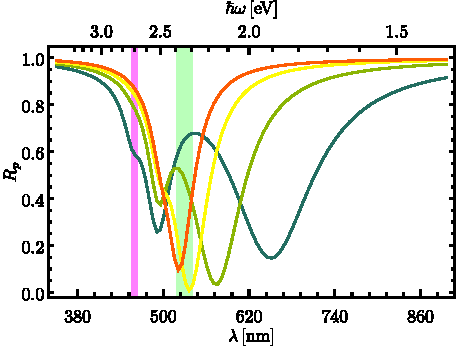
\includegraphics[scale=.75 ]{2-Resultados/figs/3-Wp4rVar/cut_angle_65_p.pdf}\end{subfigure}
	\begin{subfigure}{.01\linewidth}\caption{}\label{sfig:R-RVar-cuts}\vspace{3.75cm}\end{subfigure}\hspace*{-.5em}
	\begin{subfigure}{.45\linewidth}\centering 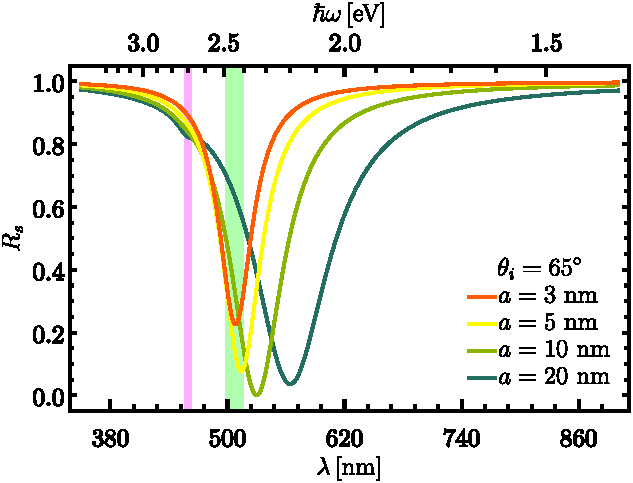
\includegraphics[scale=.75 ]{2-Resultados/figs/3-Wp4rVar/cut_angle_65_s.pdf}\end{subfigure}\vspace*{-.5em}
	\caption{Cortes a $\theta_i = 65^\circ$ de las gráficas de reflectancia de una monocapa en configuración ATR (Fig. \ref{fig:R-RVar}) de NPs esféricas de fracción de cubierta $\Theta = 0.3$ en polarización \textbf{a)} \emph{p} y \textbf{b)} \emph{s} como función de la longitud de onda $\lambda$ (escala inferior) y de la energía $\hbar\omega$ (escala superior). Los parámetros de la función dieléctrica tipo Drude para las NPs son $\omega_p = 4.3$ eV y $\gamma = 0.15$ eV y las fracciones de cubierta consideradas fueron $a$: $3$ nm, $5$ nm, $10$ nm y $20$ nm. La SP-SPR dipolar para los tamaños de partículas utilizadas corresponde la región verde entre $500$ nm y $512$ nm, mientras que la cuadrupolar corresponde a la región rosa entre $456$ nm y $462$ nm.}\label{fig:R-RVar-Cuts}
	\end{figure}	


La respuesta óptica de la monocapa a energías menores a la de la SP-SPR dipolar para las variaciones de la fracción de cubierta, así como a variaciones del radio, tienen un comportamiento semejante: a mayor cantidad de electrones libres, mayor el corrimiento al rojo; respuesta más evidente para polarización \emph{p} que \emph{s}, así como el traslape  de la SP-SPR dipolar con el presunto modo colectivo; y el valor mínimo en $R$ a la longitud de onda de la excitación para valores medios de la cantidad de electrones libres en el material. Por todo esto, se especula la existencia de un modo plasmónico semejante al PSLR reportado en  \cite{kabashin2009plasmonic} y \cite{danilov2018ultra}. 

Finalmente, se emplean las funciones dieléctricas experimentales del oro y la plata \cite{johnson1972constants} para corroborar que el presunto modo colectivo también se presenta en modelos más realistas. Para determinar las SP-SPRs de NPs de oro y plata se presenta en la Fig. \ref{fig:Q-ext} la eficiencia de extinción $Q_{ext}$ (sección transversal de extinción normalizada por la sección transversal geométrica) como función de la longitud de onda $\lambda$ (escala inferior), así como de la energía $\hbar\omega$ (escala superior) del haz incidente. Las SP-SPRs se localizan en los máximos de la $Q_{ext}$ para cada contribución multipolar: la SP-SPR dipolar se localiza en  la longitud de onda $\lambda^{(1)} = 513$ nm para el oro y $368$ nm para la plata, mientas que la SP-SPR cuadrupolar se localiza en $\lambda^{(2)} = 501$ nm para el oro y $348$ nm para la plata. %Todas las excitaciones de origen plasmónico se encunetran entre el modo dipolar $\lambda^{(1)}$ y la SPR de superficie $\lambda^{(\infty)} = \lambda^{(1)}\sqrt{2/3}$, rango de  valores que corresponden a la región gris en la Fig. \ref{fig:Q-ext}. Ya que para el oro la SPR de superficie se localiza en $418$ nm  y para la plata en $300$ nm, cualquier excitación en  la Fig. \ref{sfig:Q-ext-Au} en $\lambda<418$ para el oro no es plasmónica, así como tampoco lo son las excitaciones en la Fig. \ref{sfig:Q-ext-Ag} en $\lambda<300$ nm para la plata.


	\begin{figure}[h!]\centering
	\begin{subfigure}{.01\linewidth}\caption{}\label{sfig:Q-ext-Au}\vspace{3.75cm}\end{subfigure}\hspace*{-.5em}
	\begin{subfigure}{.45\linewidth}\centering 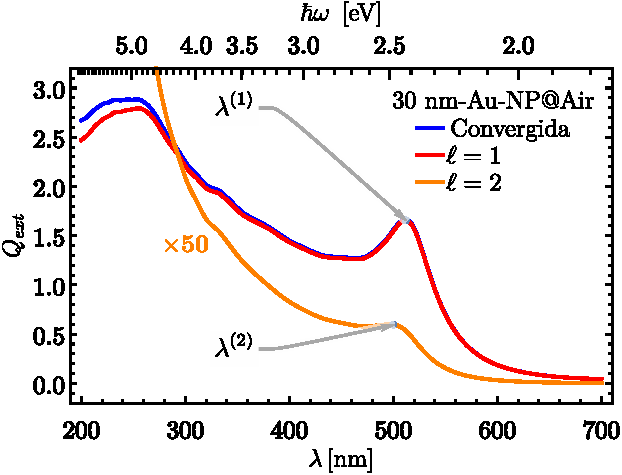
\includegraphics[scale=.75 ]{2-Resultados/figs/5-JCAu/Au_Qexr}\end{subfigure}
	\begin{subfigure}{.01\linewidth}\caption{}\label{sfig:Q-ext-Ag}\vspace{3.75cm}\end{subfigure}\hspace*{-.5em}
	\begin{subfigure}{.45\linewidth}\centering 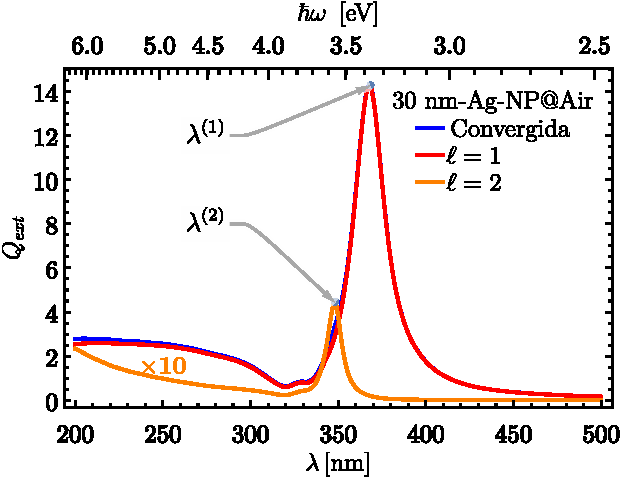
\includegraphics[scale=.75 ]{2-Resultados/figs/6-JCAg/Ag_Qexr.pdf}\end{subfigure}\vspace*{-.5em}
	\caption{Eficiencia de extinción $Q_{ext}$ de una NP individual de \textbf{a)} oro y de \textbf{b)} plata de radio $a = 30$ nm, inmersa en aire $n_m = 1$ como función de la longitud de onda $\lambda$ (escala inferior), así como de la energía $\hbar\omega$ (escala superior) del haz incidente. En azul se muestra el resultado de $Q_{ext}$ sumando seis contribuciones multipolares (convergida), en rojo se muestra la contribución del modo dipolar ($\ell = 1$) y en naranja la del modo cuadrupolar ($\ell = 2$) con un aumento de $\times 50$ para el oro y $\times 10$ para la plata. La longitud de onda de la SP-SPR dipolar $\lambda^{(1)}$ es $513$ nm para el oro y $368$ nm para la plata; la longitud de onda de la SP-SPR cuadrupolar $\lambda^{(2)}$  es $501$ nm para el oro y $348$ nm para la plata.
	% La SPR de superfice $\lambda^{(\infty)}$ para el oro se localiza en $418$ nm y para la plata en $300$ nm. La región gris delimita los valores de $\lambda$ entre $\lambda^{(\infty)}$ y $\lambda^{(1)}$, en donde se encuntran todas las excitaciones de origen plasmónico.
	 }\label{fig:Q-ext}
	\end{figure}	



En la Fig. \ref{sfig:JCAu} se calcula la reflectancia de una monocapa de NPs de oro, Fig. \ref{sfig:JCAu}, y plata, Fig. \ref{sfig:JCAg}, con un radio de $a=30$ nm y fracción de llenado $\Theta = 0.3$, inmersas en aire ($n_m = 1$) y soportadas por un sustrato con índice de refracción $n_s = 1.5$, tanto para polarización \emph{p}, gráfica \textbf{i)}, como \emph{s}, gráfica \textbf{ii)}. Las SP-SPRs para ambos materiales corresponden a las líneas punteadas verdes, para el dipolo, y las rosas para el cuadrupolo. Asimismo, todos los mínimos de $R$ corresponden a los puntos amarillos. 

	\begin{figure}[h!]\centering
	\begin{subfigure}{.01\linewidth}\caption{}\label{sfig:JCAu}\vspace{3cm}\end{subfigure}\hspace*{-1em}
	\begin{subfigure}{.45\linewidth}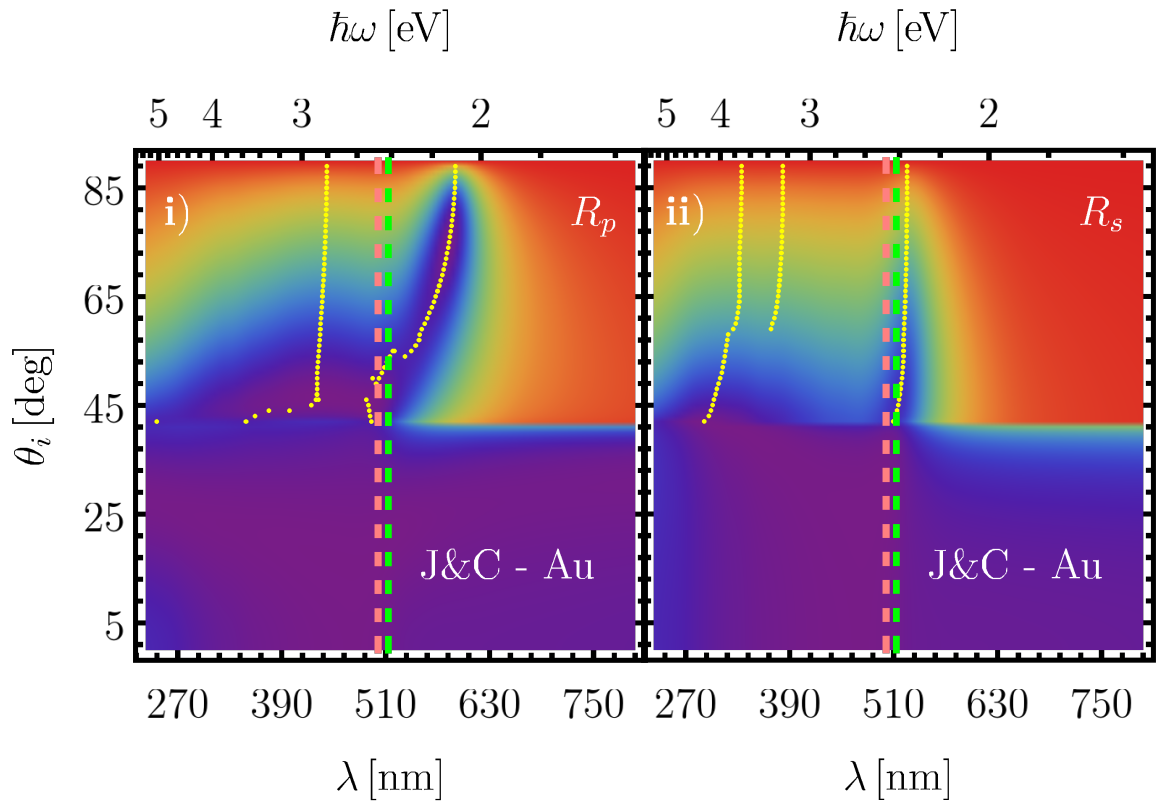
\includegraphics[width = .95\linewidth,]{2-Resultados/figs/5-JCAu/0-2D_Grid.png}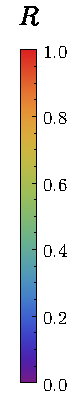
\includegraphics[scale=.6, trim={00 00 00 00}, clip]{2-Resultados/figs/0-RBar_v}
	\end{subfigure}\hspace*{1em}
	\begin{subfigure}{.01\linewidth}\caption{}\label{sfig:JCAg}\vspace{3cm}\end{subfigure}\hspace*{-1em}
	\begin{subfigure}{.45\linewidth}\centering 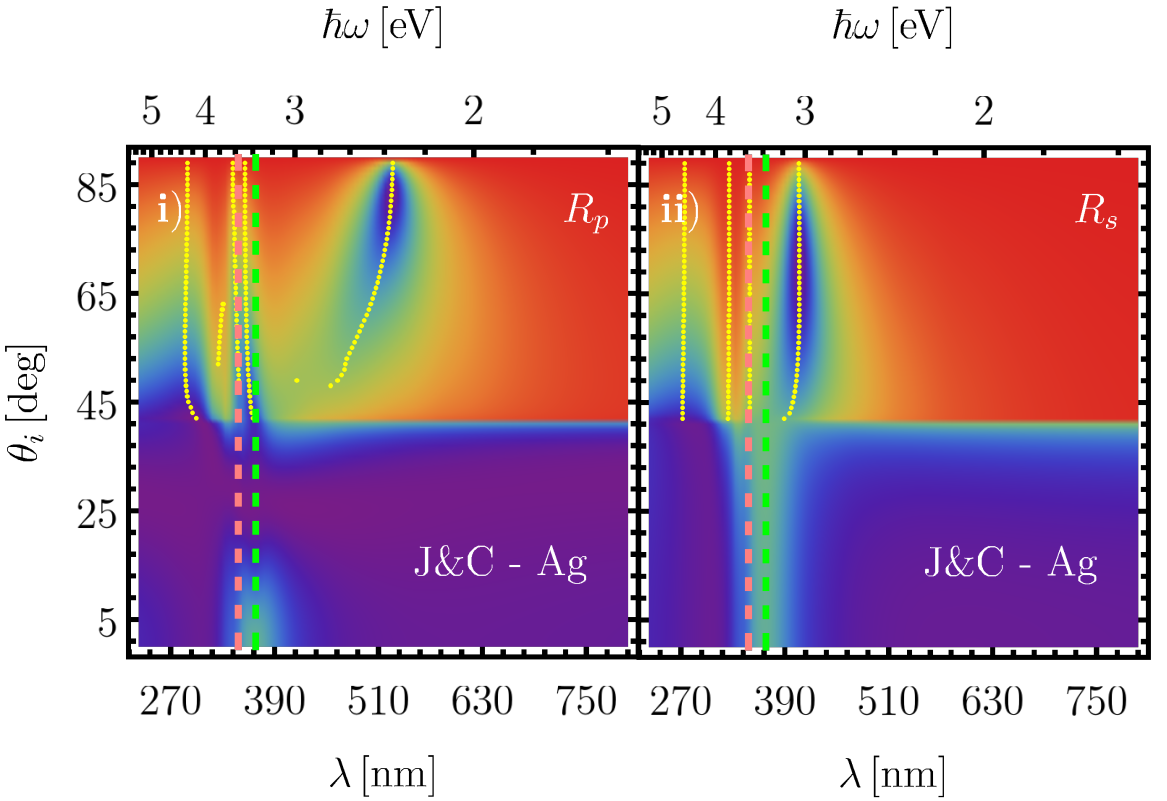
\includegraphics[width = .95\linewidth, trim={00 05 00 00}, clip]{2-Resultados/figs/6-JCAg/0-2D_Grid.png}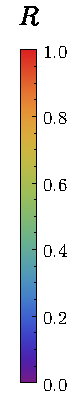
\includegraphics[scale=.6, trim={00 00 00 00}, clip]{2-Resultados/figs/0-RBar_v}\end{subfigure}
	\caption{Gráficas de reflectancia de una monocapa en configuración ATR ($\Theta = 0. 3$) como función del ángulo de incidencia $\theta_i$ y de la longitud de onda $\lambda$ para NPs de \textbf{a)} Au y \textbf{b)} Ag, calculados con los datos experimentales del índice de refracción tomados de \cite{johnson1972constants}.  Los mínimos en la reflectancia se señalizan mediante los puntos amarillos. }\label{fig:R-JC}
	\end{figure}	

Para el caso del oro, Fig. \ref{sfig:JCAu},  a ambas polarizaciones son apreciables excitaciones en $\theta_i>\theta_c \approx 41^\circ$ y  $\lambda$ menores a la longitud de onda de la SP-SPR cuadrupolar, así como una excitación a longitudes de onda mayores a la SP-SPR dipolar ($510$ nm). Para ambas polarizaciones, la excitación a las longitudes de onda mayores que la SP-SPR dipolar se comporta como el presunto modo colectivo que se analizó para una monocapa de NPs con una función dieléctrica tipo Drude, es decir, la  excitación en $\lambda>510$ nm coincide con la SP-SPR dipolar en $\theta\approx \theta_c$ y se corre al rojo conforme aumenta el ángulo de incidencia, y la separación entre el valor de la SP-SPR dipolar y la excitación en en $\lambda>510$ nm  es mayor para polarización \emph{p}, gráfica \textbf{i)}, que para polarización \emph{s}, gráfica \textbf{ii)}. Por lo anterior, la presunta respuesta colectiva es apreciable para una monocapa de NPs de oro y se traslapa con la SP-SPR dipolar.

Los resultados de la reflectancia para la monocapa de NPs de plata en la Fig. \ref{sfig:JCAg} presentan, a amabas polarizaciones, una excitación en $\theta_i>\theta_c \approx 41^\circ$ y $\lambda\approx 270$ así como una excitación en la longitud de onda $\lambda \approx 328$ nm y otra que coincide con la SP-SPR cuadrupolar en $\lambda\approx 348$ nm. La respuesta EM de la monocapa presenta una excitación en la longitud de onda cercana a la de la SP-SPR dipolar para polarización \emph{p}, gráfica \textbf{i)}, mientras que en polarización \emph{s}, gráfica \textbf{ii)} no hay una excitación cercana a la longitu de onda de la SP-SPR dipolar. Sin embargo, al igual que para la monocapa de NPs de oro, a longitudes de onda mayores a la SP-SPR dipolar, se observa una excitación que  se corre al rojo conforme aumenta el ángulo de incidencia, así como también aumenta la separación entre ésta y la SP-SPR dipolar para los resultados en polarización \emph{p}, gráfica \textbf{i)}, que en polarización \emph{s}, gráfica \textbf{ii)}. Es decir, el presunto modo colectivo es apreciable también para una monocapa de NPs de plata.

Al analizar la respuesta óptica de una monocapa con NPs modeladas mediante funciones dieléctricas tipo Drude y funciones dieléctricas experimentales, se concluye que el supuesto modo colectivo también es apreciable para modelos de NPs realistas. La excitación del supuesto modo colectivo se observa a energías menores a la excitación dipolar para una partícula individual y se corre al rojo conforme aumenta la fracción de cubierta o el radio de las NPs, es decir, conforme la cantidad de electrones libres presentes en la monocapa crece. Este modo colectivo puede sintonizarse según sean los parámetro empleados para la monocapa, radio de las NPs y fracción de cubierta, además de que puede distinguirse de la SP-SPR dipolar, a pesar del traslape observado entre ellas, dado que la extinción de luz a las longitudes de onda del presunto modo colectivo es mayor que para la SP-SPR dipolar y dado que se corre al rojo conforme la cantidad de electrones libres en la monocapa aumenta.

Para futuros cálculos en la caracterización del supuesto modo colectivo, se buscará la combinación de radios de las NPs y de fracción de cubierta en donde la extinción de luz sea máxima, así como el ancho de banda sea mínimo, para poder emplear el modo colectivo en el biosensado, al igual que la PSLR reportada en \cite{kabashin2009plasmonic} y \cite{danilov2018ultra}. Por tal motivo, se implementará la corrección por tamaño en la función dieléctrica ya que el camino libre medio de los electrones (a $273$ K) es menor a $50$ nm. Asimismo, dado que la PSLR es un modo guiado, se corroborará si el supuesto modo colectivo también es un modo guiado mediante el cálculo de la transmitancia empleando el formalismo del CSM.

